\RequirePackage{ifpdf}
\newif\ifelektroniczna
\newif\ifjednostronna

%\elektronicznatrue
\elektronicznafalse

%\jednostronnafalse
\jednostronnatrue

\ifjednostronna
    \def\strony{oneside,openany}
\else
    \def\strony{twoside,openright}
\fi

\ifpdf
    \documentclass[pdftex,12pt,a4paper,\strony,colorlinks,nocenter,noupper,crosshair]{thesis}
    \usepackage[pdftex]{graphicx}
    \pdfcompresslevel=1
\else
    \documentclass[12pt,a4paper,\strony,nocenter,noupper,crosshair]{thesis}
    \usepackage{graphicx}
\fi

\usepackage{url}
\usepackage{TitlePage}
\usepackage[utf8]{inputenc}

\def\rodzaj{Praca magisterska}

\def\wydzial{Automatyki, Elektroniki i~Informatyki}

\def\tytul{Śledzenie punktów charakterystycznych dłoni w~sekwencjach wideo}
\def\tytulpdf{Śledzenie punktów charakterystycznych dłoni w~sekwencjach wideo}

\def\autor{Autor: Wojciech Janusz Gawroński}
\def\promotor{Kierujący pracą: dr~inż. Michał Kawulok}
\def\konsultant{}
\def\data{Gliwice, Czerwiec 2013}
\def\slowakluczowe{Wizja Komputerowa,C++,OpenCV,motion tracking,machine learning,random forest}

\graphicspath{{./pictures/}}

\ifpdf
\ifelektroniczna
     \usepackage[
        pdfusetitle=true,
        pdfsubject={\tytulpdf},
        pdfkeywords={\slowakluczowe},
        pdfcreator={\autor},
        pdfstartview=FitV,
        linkcolor=blue,
        citecolor=red,
    ]{hyperref}
\fi
\fi

\usepackage{layout}

\usepackage{t1enc,amsmath}
\usepackage[OT4,plmath]{polski}
\usepackage{helvet}

%\usepackage{anysize}
%\marginsize{3cm}{2.5cm}{2.5cm}{2.5cm}%LPGD
%\setlength{\textheight}{24cm}
%\usepackage{multirow}
%\ifpdf\usepackage{pdflscape}\else\usepackage{lscape}\fi
%\usepackage{longtable}
%\usepackage{geometry}
%GATHER{thesis.bib}
%\usepackage[twoside]{geometry}
%\geometry{ lmargin=3.5cm, rmargin=2.5cm, tmargin=3cm, bmargin=3cm,
%headheight=1cm, headsep=0.5cm, footskip=0pt }
%\def\fixme#1{}

\textwidth 150mm
\textheight 225mm
\usepackage{amsfonts}
\usepackage{subfig}
\captionsetup[subfigure]{justification=centerfirst}
\usepackage{cite}
\usepackage{listings}
\lstset{language={C++},inputencoding=latin2}
\usepackage{cleardpempty}
\usepackage{float}
\usepackage{textcomp}
\def\vec#1{\ensuremath{\mathbf{#1}}}
\def\ang#1{ang.~\emph{#1}}
\def\lat#1{lac.~\emph{#1}}
\def\e{\ensuremath{\textrm{\normalfont{}e}}}
\def\degree{\ensuremath{^{\circ}}\protect}
\def\fixme#1{\marginpar{\tiny{}#1}}
\newtheorem{twierdzenie}{Twierdzenie}[chapter]
\newtheorem{wlasnosc}{Własność}[chapter]
\newtheorem{lemat}{Lemat}[chapter]
\newenvironment{dowod}{\parindent=0pt{\bf Dowód. }}{\begin{flushright}$\square$\end{flushright}}
\def\captionlabeldelim{.}
\linespread{1}
\chapterfont{\Huge\bfseries}
\sectionfont{\bfseries\Large}
\subsectionfont{\bfseries\large}
\institutionfont{\bfseries}%\mdseries}
\def\captionlabelfont{\bfseries}

\renewcommand{\figureshortname}{Rys.}
\renewcommand{\tableshortname}{Tab.}

\renewcommand\floatpagefraction{.9}
\renewcommand\topfraction{.9}
\renewcommand\bottomfraction{.9}
\renewcommand\textfraction{.1}
\setcounter{totalnumber}{50}
\setcounter{topnumber}{50}
\setcounter{bottomnumber}{50}

\newcommand{\topcaption}{%
   \setlength{\abovecaptionskip}{0pt}%
   \setlength{\belowcaptionskip}{10pt}%
   \caption}

\newcommand\scalemath[2]{\scalebox{#1}{\mbox{\ensuremath{\displaystyle #2}}}}

\newcommand{\gest}[9] {
    \subsubsection{#1}
        \begin{table}[!h]
            \begin{tabular}{l p{10cm}}
                \textbf{Tło i~kadr:}        & #2 \\
                \textbf{Kształt i~wymiary:} & #3 \\
                \textbf{Elementy składowe:} & #4 \\
                \textbf{Ułożenie dłoni:}    & #5 \\
                \textbf{Ruch i~kierunek:}   & #6 \\
                \textbf{Pozycja wejściowa:} & #7 \\
                \textbf{Punkty kluczowe:}   & #8 \\
                \textbf{Punkty pośrednie:}  & #9 \\
            \end{tabular}
            \caption{Opis gestu "#1"}
        \end{table}
}

\makeatletter
\renewcommand\fs@ruled{\def\@fs@cfont{\bfseries}\let\@fs@capt\floatc@ruled
  \def\@fs@pre{\hrule height1.0pt depth0pt \kern2pt}
  \def\@fs@post{\vskip-1.5\baselineskip\kern2pt\hrule\relax}%
  \def\@fs@mid{\kern2pt\hrule\kern2pt}
  \let\@fs@iftopcapt\iftrue}
\makeatother

\floatstyle{ruled}
\newfloat{sample}{thp}{lop}
\floatname{sample}{Przykład}

\begin{document}

\bibliographystyle{unsrt}
\frontmatter
\stronatytulowa
%\cleardoublepage
%\maketitle
%\tocbibname

\tableofcontents \listoffigures \listoftables \listof{sample}{Spis przykładów}
%\listofacros
%\input{abbrev_body}
%\newpage
%\input{spis_oznaczen}

\mainmatter
\chapter{Wstęp}\label{Chapter_Wstep}

  \section{Motywacja}\label{Section_Motywacja}

  \section{Cel}\label{Section_Cel}

\chapter{Problem śledzenia punktów charakterystycznych w~sekwencjach wideo}

  \section{Opis dziedziny problemu}\label{Section_Problematyka}
    \cite{SalientPointsTracking05}
    \cite{GoodFeaturesToTrack94}
    \cite{LucasKanadeTracker81}

  \section{Podstawowe definicje}\label{Section_Definicje}
    \cite{SalientPointsTracking05}
    \cite{GoodFeaturesToTrack94}
    \cite{LucasKanadeTracker81}

  \section{Analiza i~porównanie wybranych algorytmów}\label{Section_Algorytmy}

    \subsection{Algorytmy oparte punkty kluczowe i~analizę wybitności}\label{Subsection_SaliencyKeypoints}
      \cite{SalientPointsTracking05}

    \subsection{Algorytmy oparte o~przepływ optyczny}\label{Subsection_OpticalFlow}

      \subsubsection{Ogólny zarys algorytmów opartych o~przepływ optyczny}
      \cite{OpticalFlowNonPriori05}
      \cite{LucasKanadeTracker81}

      \subsubsection{Lucas-Kanade}
      \cite{OpenCvOpticalFlow04}

      \subsubsection{Horn-Shunck}
      \cite{HornSchunck81}

      \subsubsection{TV-L}
      \cite{TVL107}

      \subsubsection{Problem doboru cech do śledzenia dla algorytmów opartych o~przepływ optyczny}
      \cite{GoodFeaturesToTrack94}

    \subsection{Algorytm oparty o~filtr cząsteczkowy}\label{Subsection_ParticleFilter}
      \cite{ParticleFilter05}
      \cite{FingertipParticleFilter11}

    \subsection{Algorytm oparty o~decyzyjne drzewa losowe}\label{Subsection_RandomizedTrees}
      \cite{RandomizedTrees06}
      \cite{TwoStageRandomizedTrees11}

    \subsection{Algorytm oparty o~analizę łańcuchów Markova}\label{Subsection_Vitterbi}
      \cite{HandTrackingVitterbi05}

\chapter{Specyfikacja przeprowadzonych badań}\label{Chapter_SpecyfikacjaPrzeprowadzonychBadan}

  \section{Definicje gestów}\label{Section_DefinicjeGestow}

    W~ramach przeprowadzonych badań stworzono definicje poszczególnych gestów wykonywanych dłońmi użytkownika. Poniższa specyfikacja ma na celu uwspólnienie pojęć potrzebnych przy przeprowadzeniu analizy jakościowej oraz wydajnościowej.

    Wytyczne były pomocne przy procesie akwizycji oraz obróbki danych wejściowych. Wszystkie stworzone materiały testowe są zgodne z~przedstawionymi protokołami. W~zbiorze danych wejściowych możemy wyróżnić następujące definicje gestów:

    \gest{Okrąg}
         {Gest wykonywany na tle twarzy lub ciała.}
         {Okrąg o~promieniu 20 cm.}
         {Prawa dłoń.}
         {Okrąg wykonywany do kamery otwartą dłonią.}
         {Kierunek ruchu jest zgodny z~ruchem wskazówek zegara.}
         {Dłoń znajduje się na godzinie dwunastej.}
         {Punkty charakterystyczne rozmieszczone równomiernie na krawędziach dłoni.}
         {Punkty kluczowe połączone linią ciągłą rozmieszczone na okręgu co 30\degree.}

    \newpage
    \gest{Krzyż}
         {Gest wykonywany na tle twarzy lub ciała.}
         {Krzyż równoramienny o~promieniu 7 cm.}
         {Dwa, wyciągnięte palce (wskazujący oraz środkowy) prawej dłoni}
         {Kształt zarysowywany zewnętrzną strona dłoni.}
         {W~pierwszej kolejności wykonywane jest ramię pionowe, następnie palce powracają do środka i~gest wykonywany jest w~lewą stronę a~następnie w~prawo.}
         {Ustawiona dłoń znajduje się na godzinie dwunastej.}
         {Punkty charakterystyczne rozmieszczone na czubkach wyciągniętych palców.}
         {5 punktów kluczowych - cztery na krawędziach i~jeden w~środku figury.}

    \gest{Rozszerzanie}
         {Gest wykonywany w~pozycji siedzącej.}
         {W~pozycji wyjściowej, jest to kwadrat o~długości boku około 20 cm.}
         {Obie dłonie złączone czubkami palców uformowane w~gest \textit{szczypty}.}
         {Oburęczny gest rozciągania dłoni od środka.}
         {Gest powinien symulować rozciąganie niewidzialnego materiału. Kształt dłoni nie powinien ulegać zmianie w~trakcie wykonywania gestu.}
         {Obie złączone dłonie znajdują się w~środku figury na wysokości klatki piersiowej.}
         {Punkty charakterystyczne rozmieszczone równomiernie na powierzchni obu dłoni.}
         {Punkty kluczowe równomiernie rozmieszczone na przekątnej kwadratu.}

    \newpage
    \gest{Duża litera C}
         {Gest wykonywany na jednolitej i~gładkiej powierzchni.}
         {Półokrąg o~promieniu 10 cm.}
         {Palec wskazujący lewej dłoni.}
         {Zarysowanie kształtu w~kierunku przeciwnym do ruchu wskazówek zegara.}
         {Gest powinien być wykonywany przez poruszenie całej dłoni, nie tylko samego palca.}
         {Palec wskazujący na godzinie dwunastej.}
         {Punkty charakterystyczne zaznaczone na krawędziach analizowanego palca.}
         {Punkty połączone linią ciągłą rozmieszczone równomiernie na półokręgu co 30\degree.}

    \gest{Duża litera L}
         {Gest wykonywany na jednolitej i~gładkiej powierzchni.}
         {Litera "L" o~wysokości 7 cm.}
         {Złączone palce prawej dłoni.}
         {Kształt litery zarysowują czubki palców.}
         {Gest powinien być wykonywany przez poruszanie tylko złączonymi palcami, nie samą dłonią.}
         {Palce na godzinie dwunastej.}
         {Punkty charakterystyczne rozmieszczone równomiernie na górnej części dłoni.}
         {4 punkty kluczowe - na początku, na końcu, na zgięciu litery oraz dodatkowy punkt na dłuższej części litery, dokładnie w~jej połowie.}

    \newpage
    \gest{Zgniecenie}
         {Gest wykonywany na tle twarzy lub ciała.}
         {Zaciśnięcie dłoni od rozwarcia do pięści.}
         {Prawa dłoń.}
         {W~pozycji wejściowej otwarta dłoń, w~pozycji końcowej pięść zwrócona palcami do kamery, z~kciukiem na wierzchu.}
         {Gest powinien być wykonywany bez poruszania dłonią, z~jednolitą prędkością.}
         {Otwarta dłoń z~rozłożonymi palcami, skierowana wewnętrzną stroną do kamery.}
         {Punkty charakterystyczne znajdują się na czubkach palców.}
         {Punkty kluczowe rozmieszczone równomiernie na drodze wykonywanej przez każdy z~palców z~osobna.}

  \section{Akwizycja i~obróbka danych wejściowych}\label{Section_Akwizycja}

  \section{Procedura weryfikacji jakości badanego algorytmu}\label{Section_Jakosc}

    W~celu analizy i~porównania jakości poszczególnych algorytmów przygotowano zestaw parametrów, które będą badane podczas wykonania każdego z~nich. Główną rolę odgrywają tutaj \textbf{punkty kluczowe} oraz \textbf{połączenia} między nimi.

    Jakość algorytmu wyznaczana będzie na podstawie odchyleń tras oraz pozycji punktów charakerystycznych w~stosunku do pozycji punktów kluczowych oraz tras pomiędzy nimi.

    Każdy z~gestów posiada serię punktów kluczowych połączonych ze sobą liniami prostymi (w~celu symulacji gładszych połączeń np. okręgu stosuje się odpowiednią ilość punktów pośrednich). Każdy z~punktów kluczowych oprócz swojej pozycji posiada również \textit{numer klatki wideo} w~której występuje.

    W~określonych przez punkty kluczowe klatkach animacji następuje przeszukanie wszystkich dostępnych w~danej chwili czasu \textit{t} punktów charakterystycznych i~obliczana jest ich odległość od punktu kluczowego. Do porównania wybierana jest nabliższy punkt zgodnie z~metryką euklidesową.

    W~klatkach pośrednich analizowana jest odległość wszystkich punktów charakterystycznych od aktualnej \textit{trasy}. Dzięki temu, wiemy jak wygląda dystrybucja punktów charakterystycznych w~okół śledzonej trasy.

    Warto zauważyć, że taki sposób weryfikacji odporny jest na zmiany (poprzez dokładanie lub usuwanie) punktów charakerystycznych.

    Biorąc pod uwagę dwa wspomniane parametry tj. \textbf{odchylenie minimalne od punktu kluczowego w~danej klatce sekwencji wideo} oraz \textbf{wektor odchyleń punktów charakterystycznych od trasy} możemy skutecznie porównać jakość badanych algorytmów między sobą.

  \section{Procedura weryfikacji wydajności badanego algorytmu}\label{Section_Wydajnosc}

    W~celu analizy i~porównania wydajności poszczególnych algorytmów przygotowano zestaw parametrów, które obliczane będą podczas wykonania każdego algorytmu. Ujednolicenie to ma celu wypracowanie wspólnego wzorca porównawczego różnych algorytmów o~zupełnie innej zasadzie działania oraz implementacji.

    Główne parametry porównawcze opierają się na pomiarach czasu wykonania oraz własnościami statystycznymi wyciągniętymi z~pomiarów.

    Pierwszy pomar to \textbf{czas pracy algorytmu na pojedynczej klatce}. Z~wartości pomiarów dla wszystkich klatek sekwencji wideo wyciągnięte zostaną własności statystyczne tj. \textit{średnia arytmetyczna}, \textit{mediana}, \textit{odchylenie standardowe}.

    Kolejnym pomiarem jest \textbf{sumaryczny czas przetwarzania algorytmu}. Warto zauważyć, że nie będzie on nigdy mniejszy od nominalnego czasu trwania sekwencji wideo. Sumaryczny czas może być jedynie równy wartości nominalnej w~przypadku, gdy przetwarzanie pojedynczej klatki wideo odbędzie się w~czasie mniejszym bądź równym wartości niezbędnej do odczekania przed wyświetleniem następnej klatki. Czasu oczekiwania jest ściśle związany z~wartością \textit{częstotliwości klatek na sekundę} analizowanej sekwencji wideo.

    Następna wartość to \textbf{odchylenie sumarycznego czasu wykonania od czasu nominalnego} wyrażona w~procentach.

    Ostatni parametr to próba klasyfikacji wszystkich algorytmów według stopnia ich złożoności. Każdy algorytm będzie poddany analizie pod kątem wyselekcjonowanego zbioru operacji dominujących, w~celu wyznaczenia \textbf{złożoności obliczeniowej oraz pamięciowej}.
\chapter{Specyfikacja wewnętrzna}\label{Chapter_SpecyfikacjaWewnetrzna}

  \section{Wykorzystane technologie}\label{Section_Technologie}

    \subsection{C++}\label{Subsection_Cpp}
      Proces tworzenia oprogramowania przeszedł diametralne zmiany w~ostatnim dziesięcioleciu. Sformułowanie w~roku~2001 tzw. \textit{manifestu metodyk zwinnych} poruszyło klasyczny model tworzenia oprogramowania. Wspomniana ewolucja dotknęła także języki programowania. W~obecnych czasach zdecydowanie większą popularnością cieszą się języki dynamiczne (w~większości przypadków \textit{interpretowane} takie jak \textit{Ruby}, \textit{Python} lub \textit{JavaScript}), lub kompilowane do kodu pośredniego, specyficznego dla danej platformy uruchomieniowej (przykładem są języki \textit{Java} oraz \textit{C\#}).

      Przymiotniki \textit{lekki} i~\textit{zwinny}, będące podstawą wspomnianego manifestu są przede wszystkim fundamentem języków dynamicznych, ale również tych ewoluujących bardzo szybko. Język \textit{C++} zdecydowanie nie należy do tej grupy. To język statycznie typowany, o~dużej dojrzałości, czerpiący pełnymi garściami z~równie znanego poprzednika jakim jest język \textit{C}. Niestety ewoluuje on bardzo wolno (co związane jest z~dojrzałością oraz próbami zachowania kompatybilności wstecznej z~poprzednikiem), przez co stracił popularność w~obecnych czasach.

      Nadal jednak to języki kompilowane do kodu maszynowego, pod konkretną architekturę i~model procesora są w~wielu zastosowaniach niezastąpione. Tworzenie niskopoziomowego oprogramowania, tworzenie sterowników urządzeń czy aplikacji o~maksymalnych wymaganiach określonych w~zakresie wydajności to obszary gdzie język \textit{C++} i~jego poprzednicy są nadal najpopularniejszym i~najefektywniejszym wyborem. Przetwarzanie obrazów i~algorytmy wizyjne zdecydowanie należą do ostatniej grupy, przez co wszystkie najpopularniejsze biblioteki i~znaczące algorytmy są implementowane właśnie w~tych językach.

      \subsubsection{Standard ISO C++ z~roku~2003}
      Obowiązującym standardem języka \textit{C++} jest standard \textit{ISO/IEC 14882:1998} (\textit{Standard for the C++ Programming Language}) z drobnymi poprawkami zatwierdzonymi w~2003~r. (\textit{ISO/IEC 14882:2003}). W~2009 roku ogłoszono nowy standard (tzw.~\textit{C++0x}), który zaczął obowiązywać od 12 sierpnia 2011 roku, lecz wciąż oczekuje na opublikowanie (\textit{ISO/IEC 14882:2011}).

      Ostatnia wersja, wciąż oczekująca na publikację, wprowadza wiele nowości zdecydowanie ułatwiających tworzenie oprogramowania. Ujednolicono wiele koncepcji i~co najważniejsze znacznie poszerzono bibliotekę standardową co ułatwi pracę programistów i~zredukuje ilość zewnętrznych zależności niezbędnych do kompilacji. Duży udział w~rozszerzeniu biblioteki standardowej miała społeczność i~autorzy poszczególnych modułów biblioteki \textit{boost}, która jest najważniejszą i~najpopularniejszą biblioteką (wyłączając bibliotekę standardową) w~środowisku programistów \textit{C++}.

      W pracy wykorzystano stabilną i~dojrzałą wersję standardu z~roku 2003. Istnieje wiele publikacji (najpopularniejszymi są \cite{EffectiveCpp}, \cite{MoreEffectiveCpp}, \cite{EffectiveStl} oraz \cite{Alexandrescu}) oraz materiałów na temat (biblioteka \textit{MSDN} oraz dokumentacja biblioteki \textit{STL}), jak efektywnie korzystać z~dostępnej funkcjonalności i~przede wszystkim jak unikać \textit{pułapek} oraz w~jaki sposób efektywnie korzystać z~mnogości dostępnych paradygmatów i~rozwiązań udostępnionych w~specyfikacji języka.

      \subsubsection{Programowanie Obiektowe}
      Język \textit{C++} jest językiem wieloparadygmatowym, jednak dominującym paradygmatem tworzenia oprogramowania w~języku \textit{C++} jest tzw. \textit{programowanie obiektowe} (ang. \textit{Object Oriented Programming} w~skrócie \textit{OOP}). Wspomniany wyżej standard z~2003~roku posiada największe wsparcie właśnie dla tego paradygmatu, dodatkowo w~czasach największej popularności tego języka to właśnie programowanie obiektowe było najpopularniejsze.

      Koncepcja programowania obiektowego sięga języka \textit{Simula 67}, następnie dopracowano wszystkie koncepty w~języku \textit{Smalltalk}. Sam język \textit{C++}, którego pierwsza koncepcja pojawiła się w~1979 roku, intensywnie korzysta z~elementów obiektowości wprowadzonych właśnie w~języku \textit{Simula}, jak również z~języków takich jak \textit{Algol}, \textit{Ada} czy \textit{ML} \cite{CppStroustrup}.

      Programowanie obiektowe opiera się na czterech filarach, którymi są:
      \begin{itemize}
        \item \textbf{Abstrakcja} - Każdy obiekt w~systemie służy jako model abstrakcyjnego \textit{wykonawcy}, który może wykonywać pracę, opisywać i~zmieniać swój stan oraz komunikować się z~innymi obiektami w~systemie bez ujawniania, w~jaki sposób zaimplementowano dane cechy. Procesy, funkcje lub metody mogą być również abstrahowane, a~kiedy tak się dzieje, konieczne są rozmaite techniki rozszerzania abstrakcji.

        \item \textbf{Hermetyzacja} - Potocznie: ukrywanie implementacji, dokładnie: \textit{enkapsulacja}. Zapewnia, że obiekt nie może zmieniać stanu wewnętrznego innych obiektów w~nieoczekiwany sposób. Tylko własne metody obiektu są uprawnione do zmiany jego stanu. Każdy typ obiektu prezentuje innym obiektom swój interfejs, który określa dopuszczalne metody współpracy. Pewne języki~osłabiają to założenie, dopuszczając pewien poziom bezpośredniego (kontrolowanego) dostępu do stanu wewnętrznego obiektu. Ograniczają w~ten sposób poziom abstrakcji. Przykładowo w~niektórych kompilatorach języka \textit{C++} istnieje możliwość tymczasowego wyłączenia mechanizmu enkapsulacji; otwiera to dostęp do wszystkich pól i~metod prywatnych, ułatwiając programistom pracę nad pośrednimi etapami tworzenia kodu i~znajdowaniem błędów.

        \item \textbf{Polimorfizm} - Referencje i~kolekcje obiektów mogą dotyczyć obiektów różnego typu, a~wywołanie metody dla referencji spowoduje zachowanie odpowiednie dla pełnego typu obiektu wywoływanego. Jeśli dzieje się to w~czasie działania programu, to nazywa się to \textit{późnym wiązaniem} lub \textit{wiązaniem dynamicznym}. Niektóre języki udostępniają bardziej statyczne (w trakcie kompilacji) rozwiązania polimorfizmu – na przykład szablony i~przeciążanie operatorów w~\textit{C++} \cite{CppStroustrup}.

        \item \textbf{Dziedziczenie} - Porządkuje i~wspomaga polimorfizm, i~enkapsulację dzięki umożliwieniu definiowania, i~tworzenia specjalizowanych obiektów na podstawie bardziej ogólnych. Dla obiektów specjalizowanych nie trzeba redefiniować całej funkcjonalności, lecz tylko tę, której nie ma obiekt ogólniejszy. W typowym przypadku powstają grupy obiektów zwane \textit{klasami}, oraz grupy klas zwane \textit{hierarchiami dziedziczenia}. Odzwierciedlają one wspólne cechy obiektów.
      \end{itemize}

      \subsubsection{Zastosowanie programowania obiektowego w~wizji komputerowej}
      \textit{Jakość} jest subiektywnym i~niemierzalnym współczynnikiem podstawowego budulca aplikacji, jakim jest kod źródłowy. Niezmiernie ważnym jest, aby podczas procesu tworzenia oprogramowania, korzystać ze~zbioru sprawdzonych praktyk i~rozwiązań oraz pilnować spójności tworzonego produktu końcowego. Równie ważnym elementem jest dobór paradygmatu, w~jakim tworzona jest implementacja, do możliwości głównego narzędzia jakim jest język programowania i~wykorzystane biblioteki.

      Implementacja zaprezentowana w~pracy magisterskiej oparta jest na języku \textit{C++} oraz bibliotece \textit{OpenCV}, dlatego zastosowanym paradygmatem jest opisywane \textit{programowanie obiektowe}. Zgodnie z~pierwszym z~podstawowych filarów programowania obiektowego - \textit{Abstrakcją} - każda implementacja określonego algorytmu śledzenia punktów charakterystycznych jest wyabstrahowanym wykonawcą. Wszystkie implementacje korzystają z~wspólnej abstrakcyjnej klasy bazowej, natomiast detale i~sposób interakcji z~biblioteką oraz sekwencją obrazów został ukryty wewnątrz konkretnych przypadków.

      W~tym przypadku wykorzystanie abstrakcyjnej klasy bazowej to użycie \textit{Strategii}, jednego z~\textit{czynnościowych wzorców projektowych}. Zgodnie z~definicją zamieszczoną w~\cite{PatternsGoF} ten wzorzec projektowy definiuje rodzinę wymiennych algorytmów i~kapsułkuje je w postaci klas. Dzięki temu możliwe jest wymienne stosowanie każdego z~nich w~trakcie działania aplikacji niezależnie od korzystających z~nich klientów.

      Kolejną ważna abstrakcją z~punktu widzenia algorytmów przetwarzania sekwencji wideo jest klasa strumienia o~nazwie \textit{VideoStream}, która zostanie dokładnie opisana w~rozdziale \ref{Section_ImplementationDetails}. Tworzy ona abstrakcję sekwencji klatek, wraz z~możliwością wykorzystania jednego lub wielu algorytmów zgodnych z~wspomnianym wzorcem \textit{Strategii}. Dodatkowo klasa ta umożliwia otoczenie wywołań metod przetwarzających pojedynczą klatkę i~cały strumień wideo, w~celu pomiaru czasu wykonania lub ilości zużytej pamięci.

    \subsection{STL}\label{Subsection_STL}

      \subsubsection{Opis biblioteki}
      Główną częścią biblioteki standardowej języka \textit{C++} jest \textit{standardowa biblioteka szablonów} (ang. \textit{Standard Template Library}). Zawiera ona algorytmy, pojemniki, iteratory i~inne konstrukcje w~formie szablonów, przetestowane oraz gotowe do użycia przy tworzeniu oprogramowania. Głównym architektem w~początkowym stadium rozwoju tej biblioteki był \textit{Alexander Stepanov} i~na początku powstawała ona jako niezależna biblioteka rozwijana przez firmę \textit{Hewlett Packard}. Z~czasem większość przyjętych tam form wyewoluowała do formy biblioteki standardowej (w~standardzie z~roku 2003 znajduje się praktycznie większość konceptów przeniesionych ze wspomnianego pierwowzoru). Dominującym paradygmatem wykorzystywanym w~\textit{STL} jest programowanie generyczne i~dzięki temu jej składniki dobrze współpracują, z~typami wbudowanymi w~język, samą bibliotekę jak i~tymi zdefiniowanymi przez użytkownika.

      \subsubsection{Szablony}
      Fundamentem biblioteki \textit{STL} i~paradygmatu programowania generycznego (\textit{uogólnionego}) jest funkcjonalność \textit{Szablonów} dostarczana przez język \textit{C++}. Jest to możliwość tworzenia kodu programu bez wcześniejszej znajomości typów danych, na których ten będzie operował. Ten typ programowania umożliwia językom statycznie typowanym na polimorfizm typów.

      Wykorzystanie szablonów w~programach pozwala skupić się bardziej na algorytmach niż na danych jakie są przetwarzane. Użycie szablonów pozwala zredukować ilość nadmiarowego kodu ponieważ jedną funkcjonalność można zaprogramować dla wielu typów danych. Następnie kompilator w konkretnym przypadku precyzuje typ i~odpowiednio dostosowuje np. wywołania funkcji. Podczas kompilacji następuje tak zwana konkretyzacja szablonu (ang. \textit{template instantiation}), podczas której kompilator na podstawie typów danych przekazanych wzorcowi generuje kod właściwy do obsługi danego typu.

      \subsubsection{Algorytmy}
      Jedną z~podstawowych koncepcji zwartych w~\textit{STL} jest koncepcja algorytmu działającego w~oderwaniu od implementacji pojemnika. Do mediacji między pojemnikiem a~faktyczną implementacją wykorzystywany jest wzorzec \textit{Iterator} (szczegóły można znaleźć w~\cite{PatternsGoF}). Każdy z~kontenerów implementuje określony zestaw \textit{iteratorów}, które umożliwiają poruszanie się po kolejnych elementach zebranych w~kolekcji.

      Odstąpienie od powiązania abstrakcyjnego algorytmu z~implementacją pojemnika wiąże się z~wykorzystaniem \textit{idiomów}, które zostaną szerzej opisane w~jednej z~poniższych sekcji.

      Dodatkowo niektóre kolekcje posiadają własne implementacje algorytmów, przykładem może być algorytm sortowania dla kontenera list dwukierunkowych \textit{list}. W~takim przypadku zaleceniem jest wykorzystanie metody zaimplementowanej w~kontenerze, ponieważ w~większości przypadków będzie ona zoptymalizowana (dzięki wiedzy o~wewnętrznej strukturze i~implementacji danej struktury) \cite{EffectiveStl}. Wydajniejsze rozwiązanie jest obarczone w~tym przypadku powiązaniem między algorytmem a~konkretną implementacją kolekcji.

      \subsubsection{Funktory}
      Kolejnym bardzo ważnym konceptem zastosowanym w~bibliotece \textit{STL} jest abstrakcja \textit{Funktora} (ang. Functors) lub inaczej \textit{Obiektu Funkcyjnego}. Jest to klasa z~przeładowanym operatorem wywołania metody (\textit{operator()}). Możliwe jest parametryzowanie stworzonego obiektu za pomocą konstruktora oraz przechowywanie wewnętrznego stanu \textit{funktora} wewnątrz pól klasy. Ponieważ \textit{obiekt funkcyjny} i~wskaźniki na funkcje mogą być wywołane za pomocą tej samej składni mogą być stosowane zamiennie właśnie jako argumenty szablonów.

      Najpopularniejszą koncepcją zwiazaną z~\textit{funktorami} jest \textit{Predykat}. Jest to koncept zaczerpnięty z~matematyki. Jest to definicja pewnej funkcji logicznej (\textit{boolowskiej}) o~dowolnej dziedzinie i~przeciwdziedzinie będącej zbiorem wartości logicznych (\textit{prawda}, \textit{fałsz}). W~przypadku \textit{STL} wewnętrzna implementacja funktora na podstawie parametrów wejściowych podejmuje decyzje o~przypisaniu określonej wartości logicznej związanej z~przekazanymi argumentami.

      \subsubsection{Idiomy}\label{Idioms}
      Bardzo ważnym elementem podczas wykorzystywania \textit{standardowej biblioteki szablonów} jest trzymanie się określonych warunków wymaganych od typów zdefiniowanych przez użytkownika, ale także zbioru wypracowanych technik zwanych \textit{idiomami}. Pomocnym źródłem jest pozycja \cite{EffectiveStl} ilustrująca wiele przykładów wspomnianych idiomów oraz prezentująca potencjalne pułapki i~sytuacje których jako użytkownicy biblioteki powinniśmy unikać. Poniżej zamieszczony został przykład jednego z~idiomów zwanego \textit{erase-remove}, służącego do zwolnienia miejsca w~pojemniku zajmowanego przez elementy oznaczone jako usunięte (ponieważ algorytm \textit{remove} sam w~sobie nie usuwa elementów zgromadzonych w~kontenerze, jedynie przenosi je na koniec i~oznacza jako usunięte, faktyczne usunięcie może wykonać dopiero metoda \textit{erase} zaimplementowana w~określonym pojemniku).

      \begin{sample}[ht]
        \begin{verbatim}
std::vector<int> v = { 0, 1, 2, 3, 4, 5, 6 };

// Usunięcie elementów o wartości 5.
v.erase(std::remove(v.begin(), v.end(), 5), v.end());
        \end{verbatim}
        \caption{Idiom erase-remove wykorzystywany w~bibiliotece STL}
        \label{EraseRemoveIdiom}
      \end{sample}

    \subsection{OpenCV}\label{Subsection_OpenCV}

      \subsubsection{Opis biblioteki}
      \textit{OpenCV} jest jedną z~najpopularniejszych bibliotek (jeśli nie najpopularniejszą) związanych z~wizją komputerową. Zawiera funkcje wykorzystywane do obróbki obrazu, sekwencji wideo jak również i~struktury służące do uczenia maszynowego lub funkcje pomocnicze dla graficznego interfejsu użytkownika.

      Oparta jest na otwartej licencji \textit{BSD} i~jej rozwój został zapoczątkowany została przez firmę \textit{Intel} w~1999 roku. Jest ona napisana w~języku \textit{C++} i~głównym interfejs programistyczny jest dostosowany właśnie do tego języka, niemniej starsze implementacje przygotowane w~języku \textit{C} są ciągle dostępne i~istnieje możliwość ich wykorzystania.

      \textit{OpenCV} jest wieloplatformową biblioteką, w~pełni współpracującą z~systemami operacyjnymi \textit{Mac OS X}, \textit{Microsoft Windows} i~\textit{Linux}. W~momencie tworzenia pracy magisterskiej wykorzystywana była aktualnie dostępna wersja o~numerze \textit{2.4.3}. Popularność tej biblioteki przyniosła, z~pomocą społeczności, interfejsy programistyczne do praktycznie każdego popularnego języka programowania. Warto nadmienić, że obecnie wszelkiego rodzaju nowe funkcjonalności implementowane są w~języku \textit{C++}, włączając w~to wsparcie dla platform \textit{CUDA} i~podobnych.

      Dokumentacja dostępna na oficjalnej stronie internetowej jest obszerna i~wraz z~zamieszczonymi przykładami tworzy kompletny poradnik. Dodatkowo istnieje kilka pozycji literaturowych na rynkach zagranicznych, które zostały wykorzystane przy tworzeniu pracy \cite{LearningOpenCV}, \cite{OpenCVCookbook}.

      \subsubsection{Podstawowe koncepcje wykorzystywane przy pracy z~OpenCV}
      W~kontekście pracy magisterskiej biblioteka \textit{OpenCV} udostępnia wiele konceptów, które ułatwiają pracę i~pozwalają skupić się na faktycznej implementacji algorytmów. Intensywnie wykorzystywane są następujące elementy:
      \begin{itemize}
        \item Wczytywanie i~zapis różnorakich formatów sekwencji wideo.
        \item Podstawowe operacje i~filtry zdefiniowane jako pojęcia wizji komputerowej.
        \item Metody pomocnicze wspomajace implementację algorytmów śledzenia punktów charakterystycznych.
        \item Struktury ułatwiające realizację algorytmów opartych o~uczenie maszynowe.
      \end{itemize}

      Oprócz elementów zawartych w~bibliotece \textit{OpenCV} niezbędne było również wprowadzenie nowych abstrakcji ułatwiających operowanie na sekwencjach wideo (które zostały pobieżnie omówione w~sekcji \textit{Zastosowanie programowania obiektowego w~wizji komputerowej} i~zostaną omówione dokładniej w~podrozdziale \ref{Section_ImplementationDetails}).

    \subsection{Narzędzia pomocniczne}\label{Subsection_PomocniczeTechnologie}

      \subsubsection{Język R}
      \textit{GNU R} to język programowania i~środowisko do obliczeń statystycznych oraz wizualizacji wyników. \textit{R} jest podstawowym językiem programowania w bioinformatyce, ale znajduje zastosowanie w~każdej innej dziedzinie nauki wymagającej analizy statystycznej i~prezentacji wyników w~postaci różnego rodzaju wykresów.

      W~pracy magisterskiej zostały wykorzystane skrypty opierające się o~pakiety analizy statystycznej oraz prezentacji wyników pomiarów poszczególnych implementacji i~algorytmów. Poniżej zaprezentowano przykładowy skrypt, pozostałe wykresy oraz analiza statystyczna znajdują się w~rodziale \ref{Chapter_AnalizaRezultatow}.

      \begin{sample}[ht]
        \begin{verbatim}
runningTime <- rnorm(3000)
runningTimeHistogram <- hist(runningTime, breaks = 50, plot = FALSE)

plot(runningTimeHistogram, col = "red")
        \end{verbatim}
        \caption{Skrypt przygotowujący wykres czasu wykonania każdego z~algorytmów}
        \label{ChartForRunningTimePerAlgorithm}
      \end{sample}

      \subsubsection{HTML5, CSS3 i~warstwa pośrednia oparta o~NodeJS}
      Ważnym elementem jest selekcja punktów charakterystycznych w~zarejestrowanych sekwencjach wideo. W~tym celu przygotowane zostało proste narzędzie oparte w~całości na technologiach internetowych. Interfejs użytkownika został zaprojektowany i~przygotowany za pomocą \textit{HTML5} oraz \textit{CSS3}.

      Za warstwę pośrednią (spająjącą interfejs użytkownika oraz implementacje algorytmów przygotowane w~języku \textit{C++}) odpowiada środowisko uruchomieniowe \textit{NodeJS}. Jest to środowisko uruchomieniowe oprogramowywane za pomocą języka \textit{JavaScript}, które wraz z~biblioteką \textit{express} umożliwia udostępnienie statycznych zasobów (takich jak skrypty, kaskadowe arkusze stylów oraz pliki \textit{HTML}) oraz stworzenie i~również udostępnienie REST API (ang. \textit{REpresentational State Transfer Application Programming Interface}) za pomocą którego wybrane punkty, algorytm oraz wybrana sekwencja wideo przesyłane są do aplikacji napisanych w~języku \textit{C++}.

      Dzięki zastosowaniu technologii internetowych w~łatwy i~efektywny sposób stworzono interfejs użytkownika (co wymagałoby dużo większego nakładu pracy w~przypadku takiej samej implementacji w~jęzku \textit{C++}), zachowano wieloplatformowość programu pomocniczego oraz odpowiednio rozdzielono odpowiedzialności pomiędzy poszczególnymi warstwami, nie zanieczyczając domeny aplikacji (implementacja algorytmów przetwarzania sekwencji wideo) niepotrzebnymi szczegółami.

      \subsubsection{Automatyzacja pracy}
      Wszystkie procesy, zarówno dotyczące budowania aplikacji jak i~zbierania pomiarów oraz generacji wyników, są silnie zautomatyzowane. Kluczowym elementem w~tym przypadku jest system budowania \textit{SCons} oparty o~język programowania \textit{Python} oraz narzędzia pomocnicze: język skryptowy \textit{Bash} i~narzędzie \textit{FFmpeg}.

      Automatyzacja procesu budowania ułatwia w~znacznym stopniu proces tworzenia oraz testowania oprogramowania, która w~przypadku języka \textit{C++} oraz większych aplikacji może być kłopotliwa. Dzięki zastosowaniu systemu budowania opartego o~język interpretowany (w~tym przypadku \textit{Python}) ułatwia wykorzystanie skryptów budowania na innym systemie operacyjnym niż został oryginalnie przewidziany - jedyną dodatkową zależnością będzie interpreter. W~przypadku zastosowania klasycznego systemu budowania opartego o~program \textit{Makefile}, ponowne wykorzystanie na platformie \textit{Windows} byłoby znacznie utrudnione - \textit{SCons} kosztem jednego dodatkowego elementu sprowadza ponowne wykorzystanie skryptów budowania do instalacji wspomnianej zależności. Poniżej zaprezentowano wycinek skryptu budowania dla opisywanego narzędzia.

      \begin{sample}[ht]
        \begin{verbatim}
environment = Environment(CPPFLAGS = "-O3 -Wall")

openCV = [ "opencv_core",
           "opencv_highgui",
           "opencv_video",
           "opencv_imgproc" ]

libraries = openCV + [ "common" ]
exporter = [ "./domain/exporter/main.cpp" ]

# ...

environment.Program("./bin/export-first-frame",
                    exporter,
                    LIBS = libraries,
                    LIBPATH = "./bin")
        \end{verbatim}
        \caption{Fragment skryptu automatyzującego procesu budowania}
        \label{BuildingProcessScript}
      \end{sample}

      Uruchamianie, akwizycja danych testowych w~początkowej fazie tworzenia oprogramowania oraz konwersja wideo do najróżniejszych formatów została zrealizowana za pomocą skryptów \textit{Bash} i~narzędzia \textit{FFmpeg}. Dzięki krótkim skryptom (kilka linii kodu źródłowego) udało się sprowadzić do minimum procesy, które programista musiałby wykonywać ręcznie. Poniżej znajduje się fragment jednego ze skryptów pomocniczych.

      \newpage
      \begin{sample}[ht]
        \begin{verbatim}
#!/bin/sh

# ...

for file in *.avi; do
  ffmpeg -i $file -r 25
         -f webm -b:v 20M videos-converted/${file%%.*}.webm
done
        \end{verbatim}
        \caption{Fragment skryptu konwertującego pliki AVI do formatu WEBM}
        \label{UtilityScript}
      \end{sample}

  \section{Szczegóły techniczne implementacji wybranych algorytmów}\label{Section_ImplementationDetails}

\chapter{Specyfikacja zewnętrzna}\label{Chapter_SpecyfikacjaZewnetrzna}
\chapter{Analiza wyników badań}\label{Chapter_AnalizaRezultatow}

  \section{Opis wygenerowanych zbiorów i~rezultatów}\label{Section_Results}
    Zanim zostaną dokładnie omówione i~przeanalizowane wyniki przeprowadzonych badań, warto przybliżyć kilka szczegółów dotyczących zebranych rezultatów.

    Wszystkie wyniki zostały zebrane z~plikach z~rozszerzeniem JSON (są to samoopisujace się pliki tekstowe ogólnego przeznaczenia, oparte na strukturze słownika typu \textit{klucz} - \textit{wartość}). Rozmiar wygenerowanych danych wynosi $4,1$ MB, co jak na dane czysto tekstowe jest dość dużą liczbą (ponad 4 miliony znaków).

    Czas trwania podstawowych testów (analiza wszystkich zebranych próbek - 3 różne algorytmy o~domyślnych parametrach, 10 osób po 6 gestów) to ponad dwie i~pół godziny. Dla wyspecjalizowanych przypadków czas przetwarzania wyniósł trzy i~pół godziny (wybrane parametry dla 3 algorytmów na 2 najlepszych jakościowo próbkach 2 gestów). Przypadki dodatkowe zostały zebrane w~pliku \textit{parametrized.json} umieszczonym w~katalogu głównym kodu źródłowego.

    W~przypadku algorytmu opartego na uczeniu maszynowym, rozmiar wygenerowanych zbiorów treningowych dla domyślnych parametrów (las złożony z~5~drzew losowych, 200 punktów charakterystycznych, wymiar boku kwadratowej łaty - 20 pikseli) wyniósł dokładnie $43$ GB. Czas generacji został uwzględniony w~powyższym akapicie.

    Rezultaty zostały zebrane za pomocą 64 wykresów, analizujących cztery różne obszary porównawcze, tj.:
    \begin{itemize}
      \item Zużycie pamięci wirtualnej i~fizycznej.
      \item Wydajność (czasy przetwarzania klatki animacji oraz czas dodatkowych operacji niezbędnych do obliczeń).
      \item Narzut czasowy obliczeń, wprowadzony do nominalnego czasu trwania sekwencji wideo.
      \item Jakość wygenerowanej ścieżki w~stosunku do wyznaczonych manualnie punktów i~ścieżek kluczowych.
    \end{itemize}

    W~kolejnych sekcjach zostały szczegółowo omówione wyniki oraz przedstawione wnioski dla każdego z~analizowanych obszarów.

  \section{Wnioski i~wyniki związane z~zużyciem pamięci badanych algorytmów}\label{Section_Memory}

    Zaimplementowane algorytmy posiadają zupełnie trzy odrębne profile pamięciowe co zamieszczone zostało na wykresach \ref{fig:MemoryUsagePersonAC} oraz \ref{fig:MemoryUsagePersonGC}, reprezentujących dwie odrębne próbki. W~przypadku metod opartych o~rodzinę algorytmów przepływu optycznego wartość zużywanej pamięci nie różni się pomiędzy poszczególnymi próbkami. Dla trzeciego algorytmu zużycie waha się w~przedziale od $350$ do $800$ MB dla pamięci wirtualnej i~dla pamięci fizycznej w~przedziale od $150$ do $600$ MB. Widać wyraźnie, że najwięcej pamięci pochłania implementacja opierająca się algorytmie wykorzystującym las drzew losowych i~ilość zaalokowanej pamięci zależy ściśle od przygotowanej bazy treningowej oraz parametrów próbki wideo.

    \begin{figure}[!ht]
      \centering
      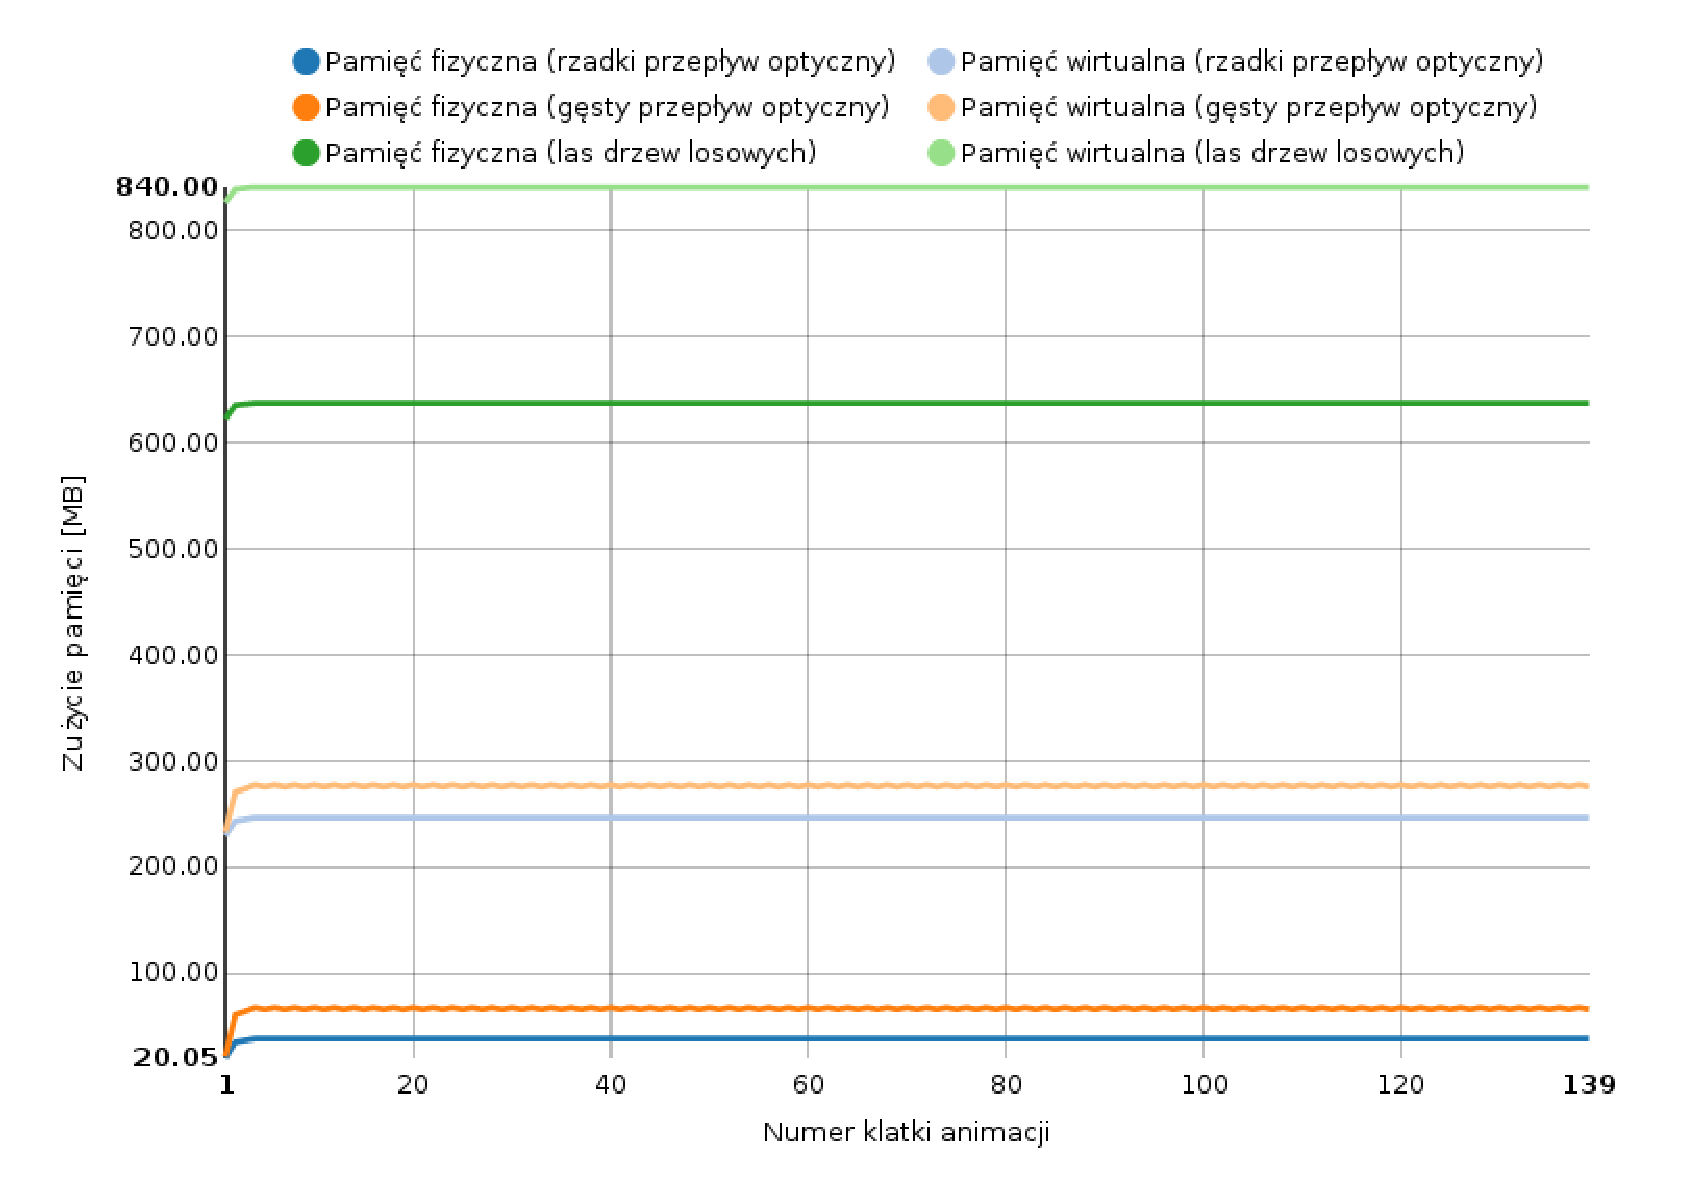
\includegraphics[width=14cm]{charts/memory/PersonAC}
      \caption[Wykres zużycia pamięci dla próbki o nazwie Person\_A\_C]
              {Wykres zużycia pamięci dla próbki o nazwie \textit{Person\_A\_C}}
      \label{fig:MemoryUsagePersonAC}
    \end{figure}

    W~przypadku gęstego przepływu optycznego zużycie pamięci fizycznej nie przekracza $80$ MB, dla implementacji algorytmu opartego o~metodę \textit{LK} osiąga wartość co najwyżej $50$ MB. Oba algorytmy są zdecydowanie oszczędniejsze od trzeciej zapronowanej implementacji.

    \begin{figure}[!ht]
      \centering
      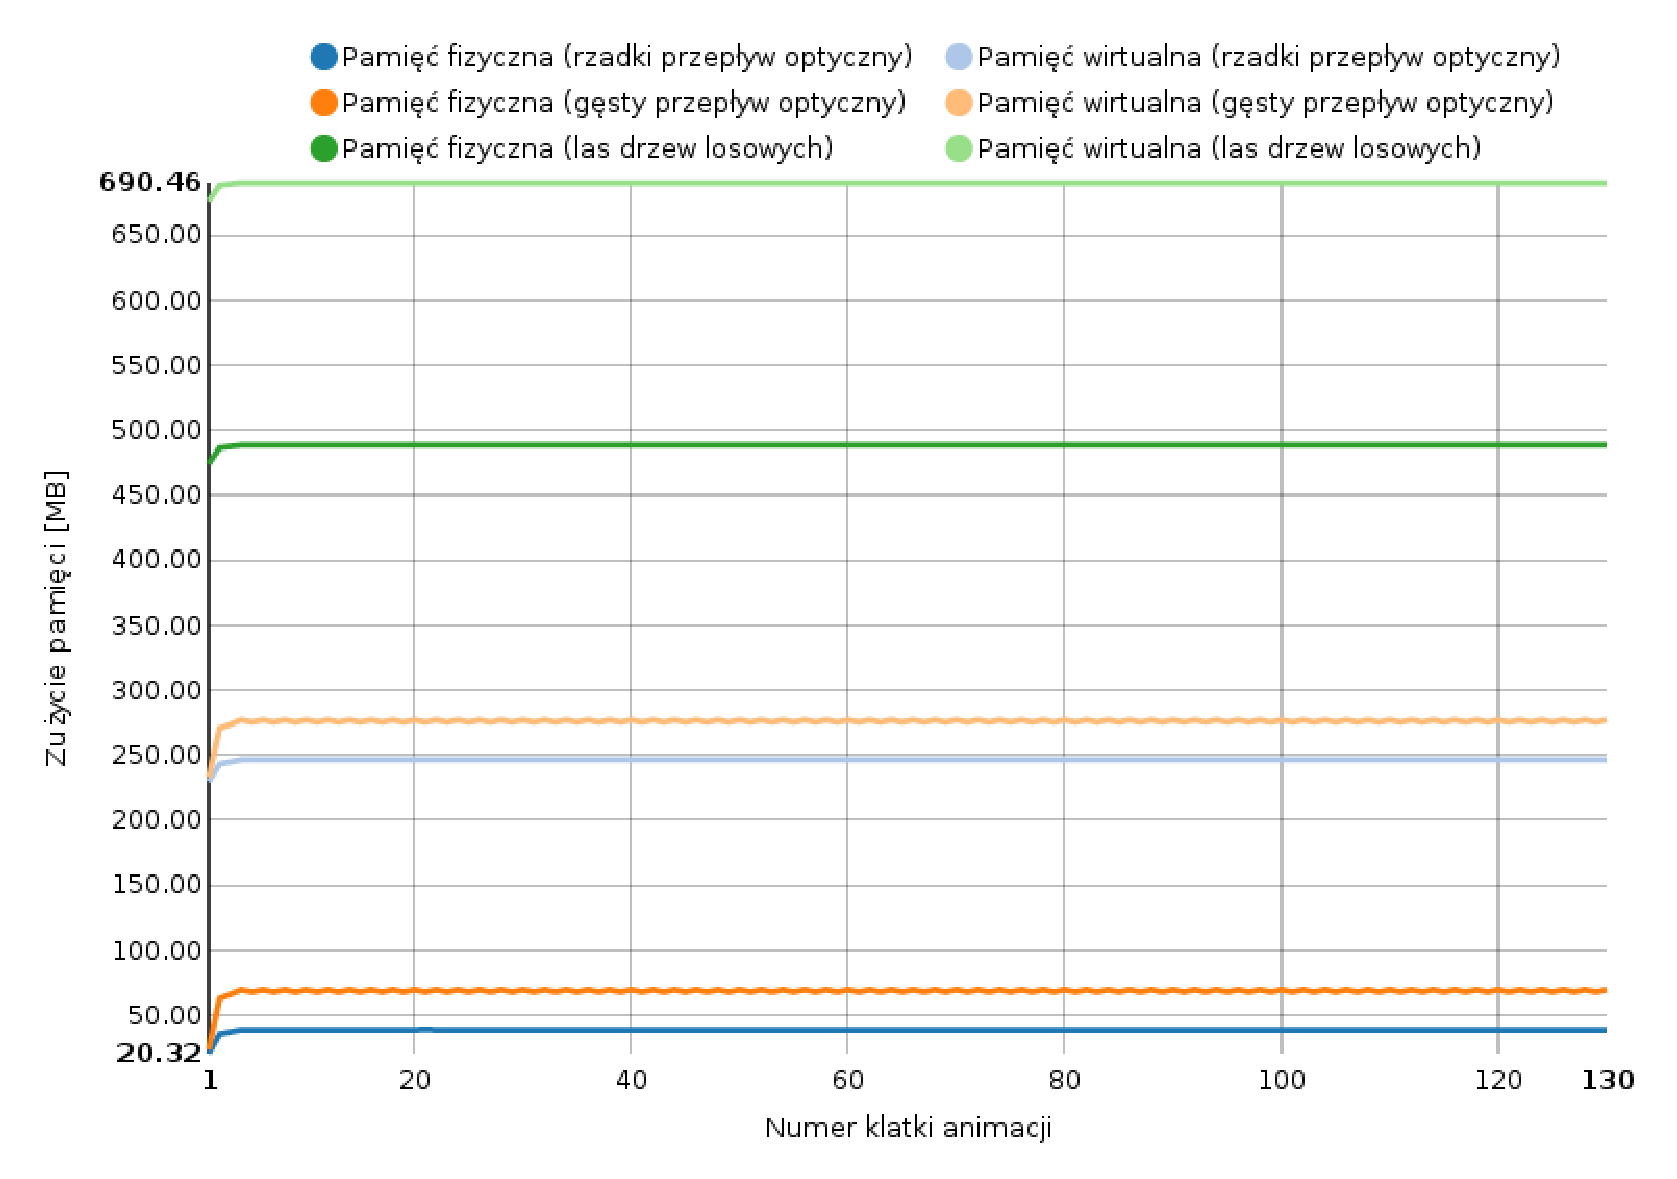
\includegraphics[width=14cm]{charts/memory/PersonGC}
      \caption[Wykres zużycia pamięci dla próbki o nazwie Person\_G\_C]
              {Wykres zużycia pamięci dla próbki o nazwie \textit{Person\_G\_C}}
      \label{fig:MemoryUsagePersonGC}
    \end{figure}

    Algorytm gęstego przepływu optycznego posiada jedną wadę - mimo stosunkowo niewielkiego zużycia pamięci, na wykresie \ref{fig:OpticalFlowsMemoryUsage} został zaprezentowany piłokształtny przebieg, ciągłej alokacji i~zwalniania od 2 do 4 MB bufora pamięci pomiędzy poszczególnymi klatkami sekwencji wideo. Nie jest to korzystne zjawisko i~jego eliminacja na pewno wpłynie pozytywnie na całkowitą wydajność.

    \begin{figure}[!ht]
      \centering
      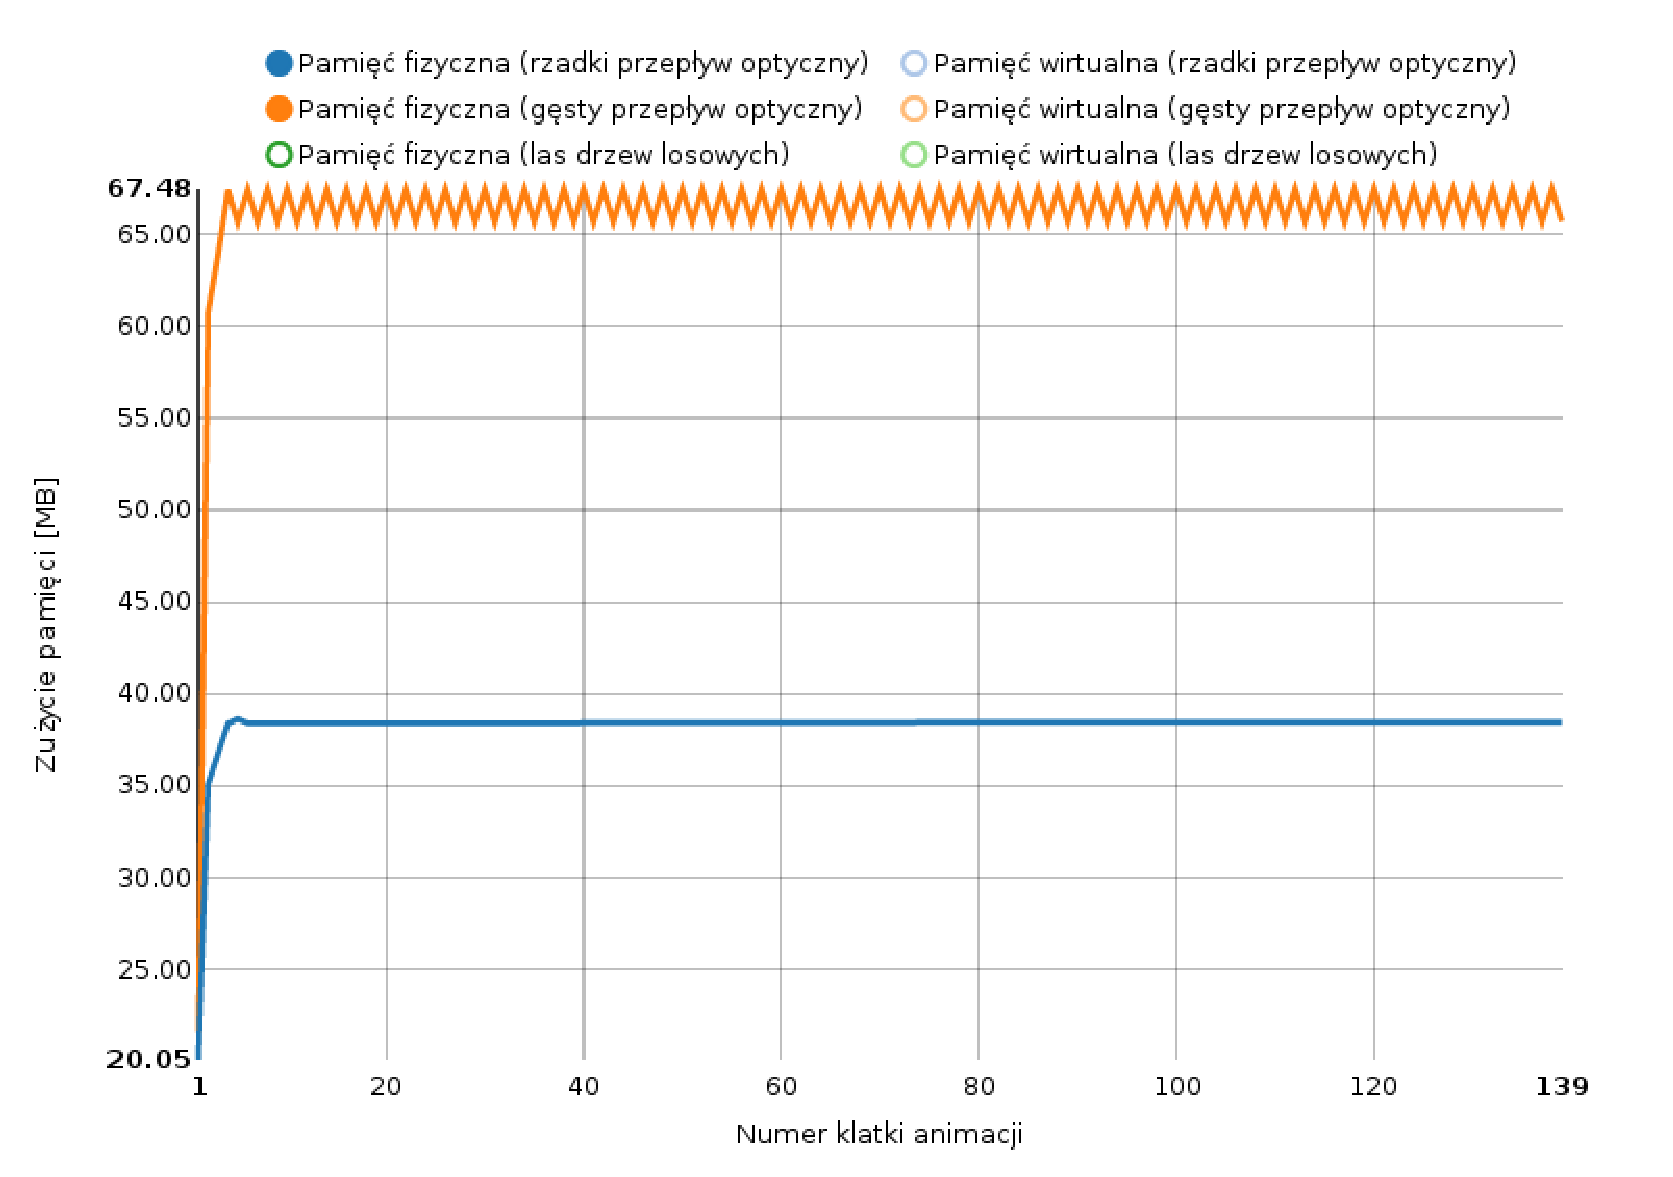
\includegraphics[width=14cm]{charts/memory/OpticalFlows}
      \caption[Wykres zużycia pamięci dla algorytmów przepływu optycznego]
              {Wykres zużycia pamięci dla algorytmów przepływu optycznego}
      \label{fig:OpticalFlowsMemoryUsage}
    \end{figure}

    W~przypadku algorytmu opartego o~las drzew losowych zużycie pamięci liniowo zależy od ilości wytrenowanych drzew wykorzystanych do budowy klasyfikatora. Zależność została zaprezentowana na rysunku \ref{fig:RandomForestTrackerPerTrainedTreesAmount}. Jednocześnie można zauważyć, że różnica pomiędzy minimalnym i~maksymalnym zużyciem pamięci jest niewielka co oznacza, że proces potrzebuje dużej ilości pamięci, ale nie jest algorytmem intensywnym w~operacje przydzielania i~zwalniania zasobów.

    \begin{figure}[!ht]
      \centering
      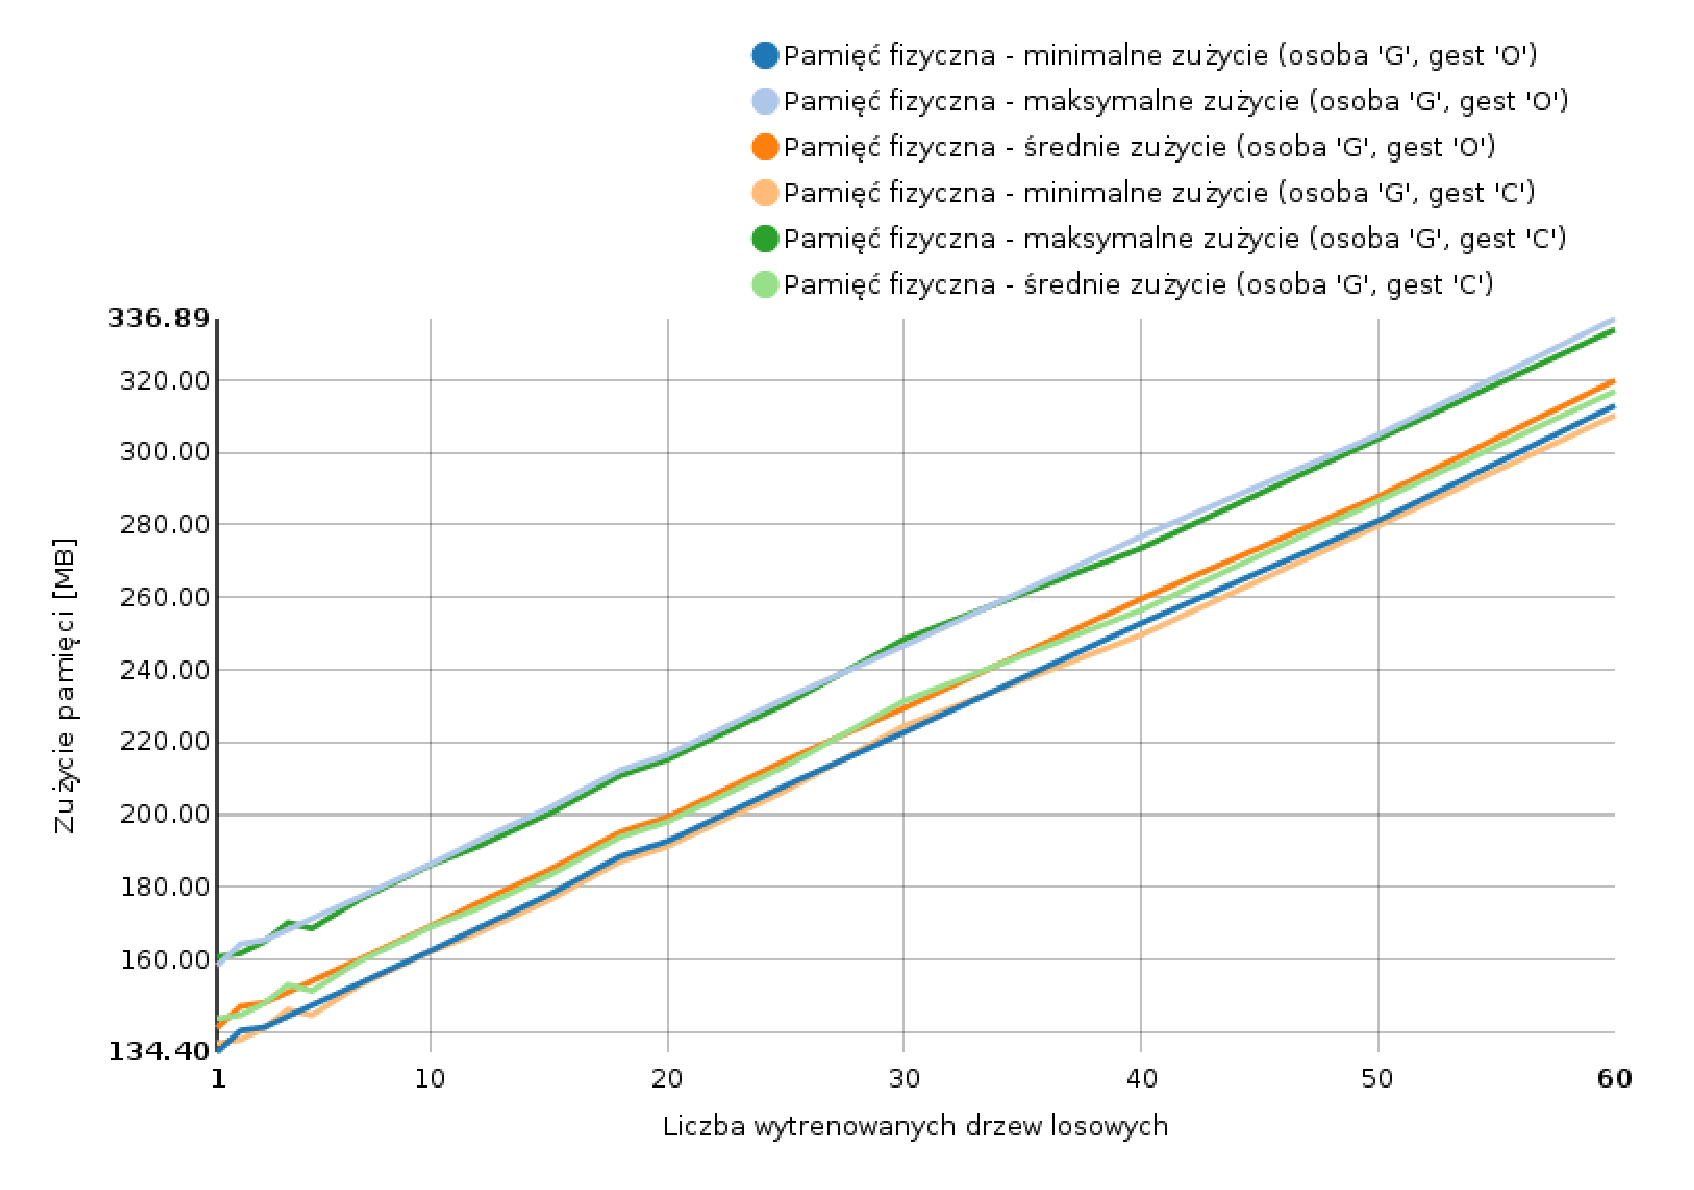
\includegraphics[width=14cm]{charts/memory/RandomPerTrainedTree}
      \caption[Wykres zużycia pamięci dla algorytmu lasu drzew losowych w~zależności od liczby wytrenowanych drzew]
              {Wykres zużycia pamięci dla algorytmu lasu drzew losowych w~zależności od liczby wytrenowanych drzew}
      \label{fig:RandomForestTrackerPerTrainedTreesAmount}
    \end{figure}

    Rzadki przepływ optyczny charakteryzuje się niewielkimi wahaniami zużycia pamięci w~zależności od minimalnej odległości pomiędzy śledzonymi punktami charakterystycznymi (jak można było przypuszczać, im większa odległość tym mniejsze zużycie pamięci). Na wykresie \ref{fig:SparseOpticalFlowPerMinimalDistanceBetweenPoints} widać, że fluktuacje mieszczą się w~przedziale o~szerokości około $30$ MB i~nie przekraczają wartości $63$ MB, co nie jest bez znaczenia w~środowisku z~ograniczonymi zasobami pamięciowymi (np. systemy wbudowane lub urządzenia mobilne). Z trzech porównywanych implementacji, metoda oparta o~algorytm \textit{LK} w~wariancie piramidalnym jest najoptymalniejsza pod względem zużycia pamięci.

    \begin{figure}[!ht]
      \centering
      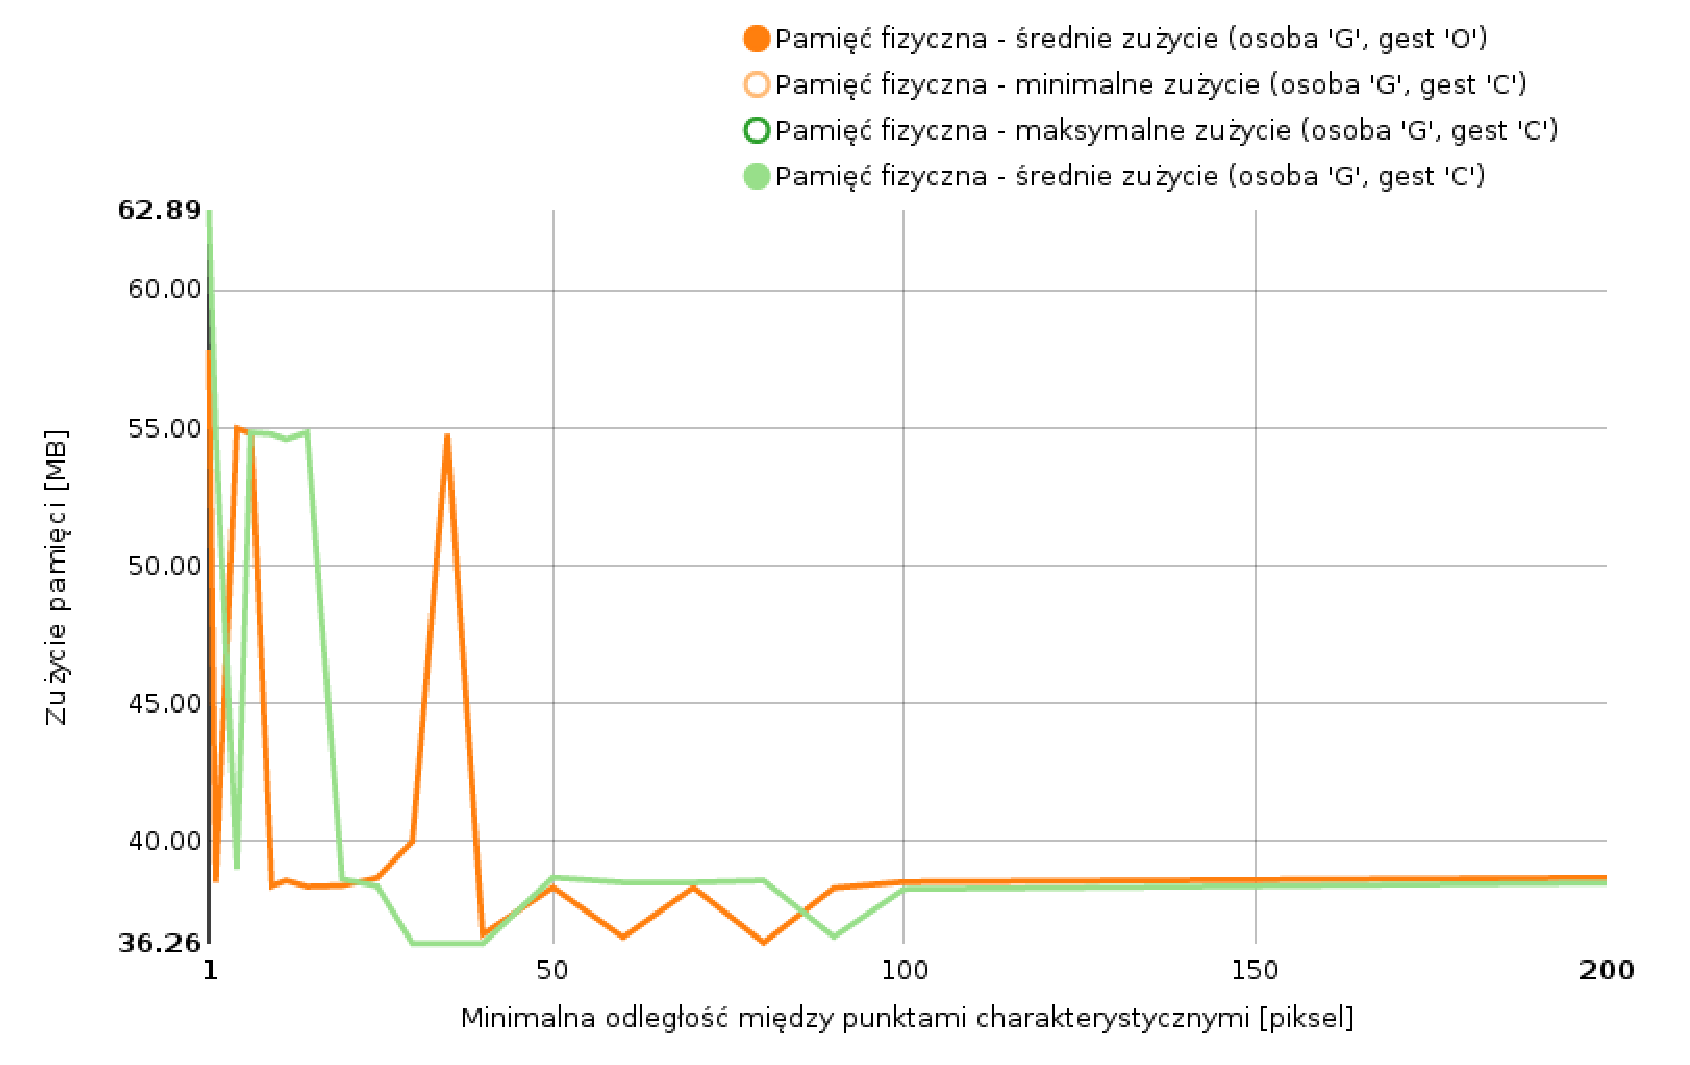
\includegraphics[width=14cm]{charts/memory/SparsePerMinimalDistance}
      \caption[Wykres zużycia pamięci dla rzadkiego przepływu optycznego w~zależności przyjętej minimalnej odległości pomiędzy punktami charakterystycznymi]
              {Wykres zużycia pamięci dla rzadkiego przepływu optycznego w~zależności przyjętej minimalnej odległości pomiędzy punktami charakterystycznymi}
      \label{fig:SparseOpticalFlowPerMinimalDistanceBetweenPoints}
    \end{figure}

    \begin{figure}[!ht]
      \centering
      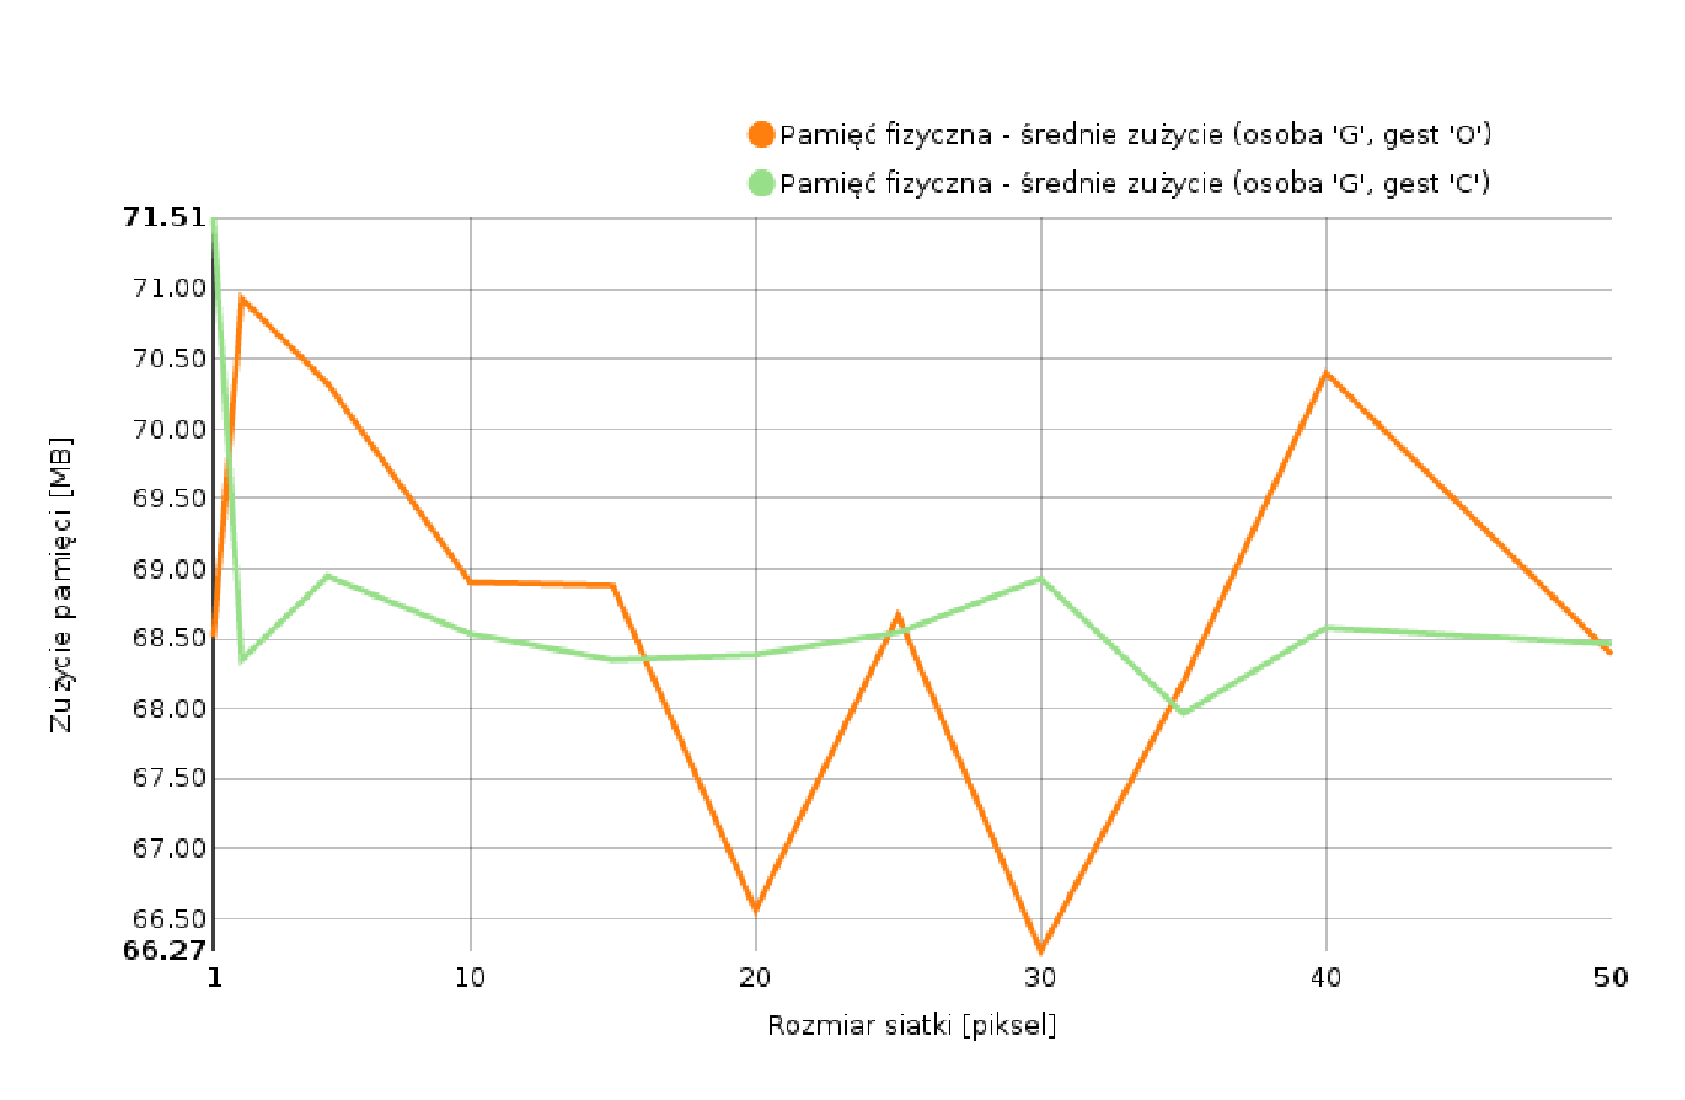
\includegraphics[width=14cm]{charts/memory/DensePerMapOverlaySize}
      \caption[Wykres zużycia pamięci dla gęstego przepływu optycznego w~zależności od gęstości siatki]
              {Wykres zużycia pamięci dla gęstego przepływu optycznego w~zależności od gęstości siatki}
      \label{fig:DenseOpticalFlowPerMapSize}
    \end{figure}

    \newpage

    W~wariancie gęstym zależnym od rozmiaru przyjętej siatki, przepływ optyczny charakteryzuje się wyższym zużyciem pamięci (maksymalnie około $72$ MB), jednak same wahania są stabilniejsze, mieszczą się w~przedziale o~szerokości około $5$ MB. Widać, że zwiększenie wymiarów siatki (intuicyjnie, rozrzedzenie jej) nie zawsze idzie w~parze z~malejącym zużyciem pamięci. Warto jednak zauważyć, że wahania odbywają sie w~bardzo niewielkim zakresie.

    Mimo wyższego zużycia całościowego, jego wartość nadal nie jest zbyt wysoka i~algorytm gęstego przepływu optycznego sprawdzi się w~środowisku z~ograniczonymi zasobami pamięciowymi.

  \section{Wnioski i~wyniki badania wydajności}\label{Section_Timing}

  \section{Wnioski i~wyniki związane z~wprowadzonym narzutem czasowym}\label{Section_Overhead}

  \section{Wyniki i~wnioski weryfikacji jakości badanych algorytmów}\label{Section_Quality}

  \section{Proponowane usprawnienia}\label{Section_Usprawnienia}

    Na podstawie analizy zawartej w~powyższych podrozdziałach nasuwa się kilka wniosków i~potencjalnych ulepszeń. Zostały one zebrane i~omówione poniżej.

    \begin{itemize}
      \item \textbf{Rozszerzenie sposobu budowania bazy treningowej dla algorytmu wykorzystującego las drzew losowych.}

      Aby zwiększyć jakość klasyfikacji oraz jeszcze bardziej uodpornić algorytm na zmianę kształtu śledzonej dłoni należy udoskonalić proces generacji danych wejściowych. Potencjalnym rozszerzeniem może być wykorzystanie nie tylko pierwszej klatki animacji, do generowania zbioru danych treningowych. Innym rozszerzeniem, może być dodanie kolejnych transformacji źródłowej klatki animacji (np. celowego zniekształcenia perspektywy lub tzw. \textit{rybiego oka} oraz dodatkowego rodzaju szumu).

      \item \textbf{Optymalizacja zużycia pamięci dla algorytmu przepływu optycznego gęstego.}

      W~sekcji \ref{Section_Memory} podczas omawiania zużycia pamięci dla wspomnianego algorytmu dało się zauważyć ciągłą zmianę zużywanej pamięci fizycznej (i~w konsekwencji także wirtualnej, rysunek \ref{fig:OpticalFlowsMemoryUsage}). Ciągła alokacja i~zwalnianie przydzielonych zasobów negatywnie wpływa na czas przetwarzania klatki sekwencji wideo. Narzut ten, może zostać zniwelowany za pomocą zmiany sposobu alokacji pamięci np. poprzez zastosowanie wielokrotnie wykorzystywanej i~współdzielonej puli pamięci.

      \item \textbf{Optymalizacja zużycia pamięci dla algorytmu opartego o drzewa losowe.}

      Omawiany algorytm podczas pracy wykorzystuje bardzo dużo (w~odniesieniu do pozostałych dwóch metod) pamięci fizycznej. W~celu zwiększenia przydatności algorytmu należy przeprowadzić proces optymalizacji zużycia pamięci.

      \item \textbf{Przyspieszenie procesu uczenia, odczytu oraz zapisu bazy treningowej.}

       W~obecnej implementacji przy generacji, zapisie oraz odczycie bazy treningowej wykorzystywany jest jeden wątek (w~konsekwencji również jeden procesor). W~oryginalnym algorytmie (opisanym w~pracy \cite{RandomizedTrees06}) autorzy proponują rozdzielenie omawianych etapów pracy algorytmu na cztery wątki, co zdecydowanie lepiej wykorzystuje możliwości współczesnego sprzętu.
    \end{itemize}

\chapter{Podsumowanie}\label{Section_Podsumowanie}

W~ramach pracy magisterskiej omówiono i~przeprowadzono badania wydajnościowe oraz jakościowe implementacji trzech algorytmów śledzenia punktów charakterystycznych pod kątem wykorzystania ich do analizy ruchu dłoni.

Zebrane rezultaty pozwoliły na jednoznaczne określenie przydatności poszczególnych algorytmów w~badanym obszarze.

Oprócz zaproponowanych implementacji, badań oraz~analizy zostały również zaproponowane usprawnienia i~potencjalne rozszerzenia, które zwiększą jakość oraz poprawia wydajność omawianych metod.

\addcontentsline{toc}{chapter}{\bibname}
\bibliography{MainDocument}

\renewcommand{\appendixname}{Dodatek}
\appendix
\chapter{Środowisko uruchomieniowe}\label{Chapter_EnvironmentAppendix}
  \section{Zależności}\label{Section_Dependencies}

  Poniżej zebrane zostały zależności niezbędne do uruchomienia środowiska uruchomieniowego:
  \begin{itemize}
    \item Interpreter języka \textit{Python} w~wersji z~rodziny \textit{2.7.x},
    \item Narzędzie budowania \textit{SCons},
    \item Kompilator języka C++ (w~zależności od systemu operacyjnego \textit{GCC} lub \textit{Microsoft Visual Studio 2012 C++ Compiler}),
    \item Biblioteka \textit{OpenCV} w~wersji \textit{2.4.3} skompilowana pod odpowiedni system operacyjny,
    \item Środowisko uruchomieniowe \textit{node.js} w~wersji z~rodziny \textit{0.8.x},
    \item Współczesna i~aktualna przeglądarka internetowa (najlepiej \textit{Mozilla Firefox} lub \textit{Google Chrome}).
  \end{itemize}

  \section{Instalacja i~uruchomienie}\label{Section_Installation}

  Po zainstalowaniu niezbędnych środowisk, narzędzi oraz bibliotek dostarczonych wraz z~kodem źródłowym na nośniku dołączonym do pracy, należy skopiować katalog \textit{src} w~dowolne miejsce na dysku twardym, gdzie nasz użytkownik posiada prawa zapisu.

  Aby rozpocząć badanie, dla obu platform (\textit{Microsoft Windows} oraz \textit{Linux}), znajdując się w~powyższym katalogu należy wykonać z~linii poleceń komendę \textit{node run-tests.js}, który ustawia odpowiednie zmienne środowiskowe i~przystępuje do kompilacji oraz uruchomienia badań.

  Rezultaty badań, wraz z~wykresami po zakończeniu procesu znajdą się w~katalogu \textit{assets} wewnątrz uprzednio skopiowanego katalogu.

\end{document}